\section{Comprendre les outils de métamodélisation d'Eclipse EMF}

Pour la prise en main des outils d'Eclipse on étudie le cas d'un modèle de procédé vu en td. Ce modèle suit un métamodèle simplePDL. Une première version de ce métamodèle est la suivante :

\begin{figure}[h]
   \centering
   \subfloat[modèle du sujet]{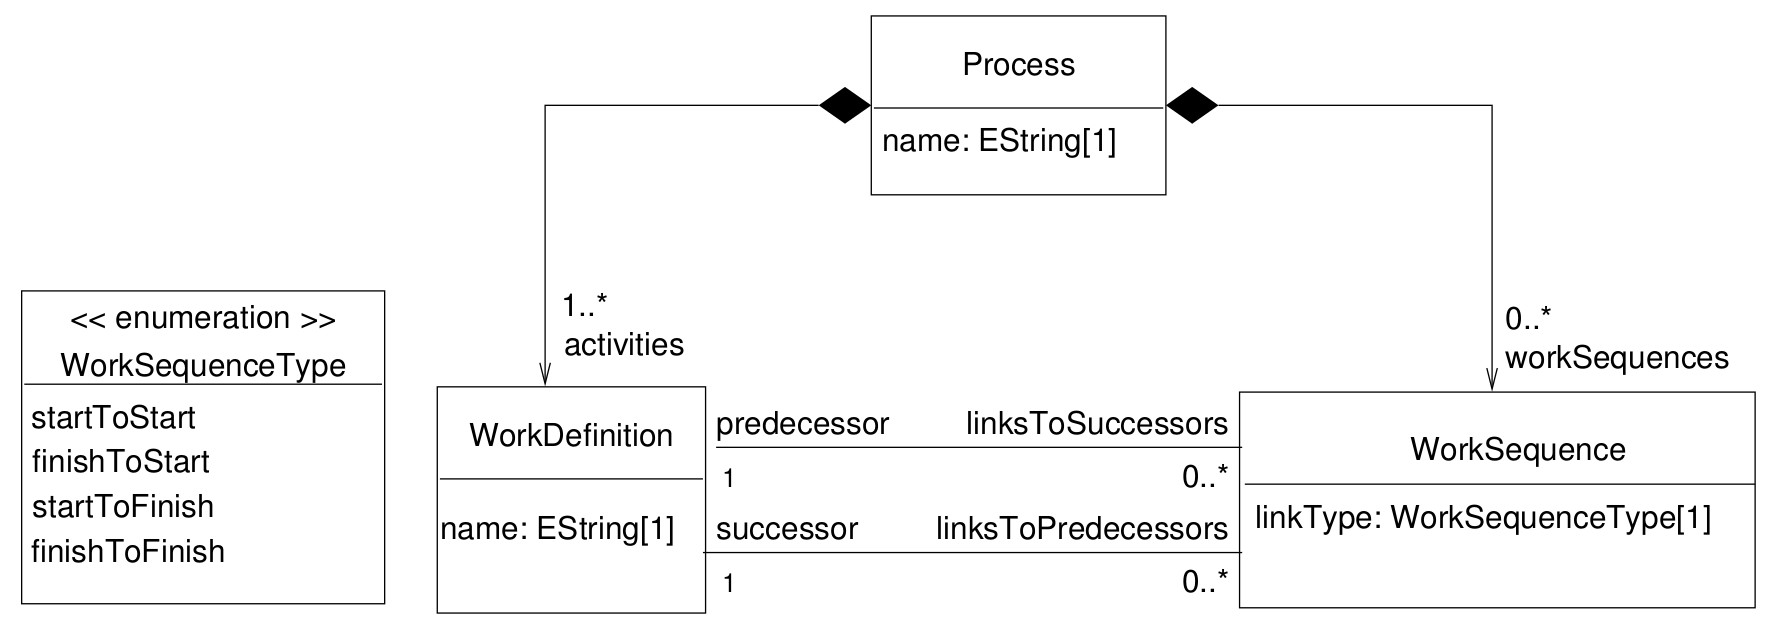
\includegraphics[width = 0.5\textwidth]{../Images/tp2/tp2_1-1.png}}
   \subfloat[diagramme du modèle ecore]{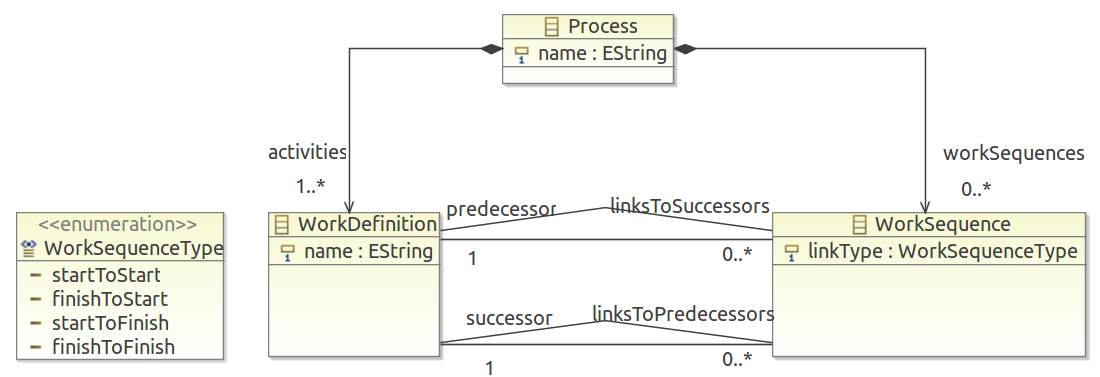
\includegraphics[width = 0.5\textwidth]{../Images/tp2/tp2_1-2.png}}
   \caption{Première version du métamodèle SimplePDL}
   \label{pdlv1}
\end{figure}

On utilise ensuite ce modèle avec l'éditeur réflexif (\textit{Create dynamic instance}) pour créer le modèle de procédé vu en td :

\begin{figure}[h]
   \centering
   \subfloat[Modèle de procédé]{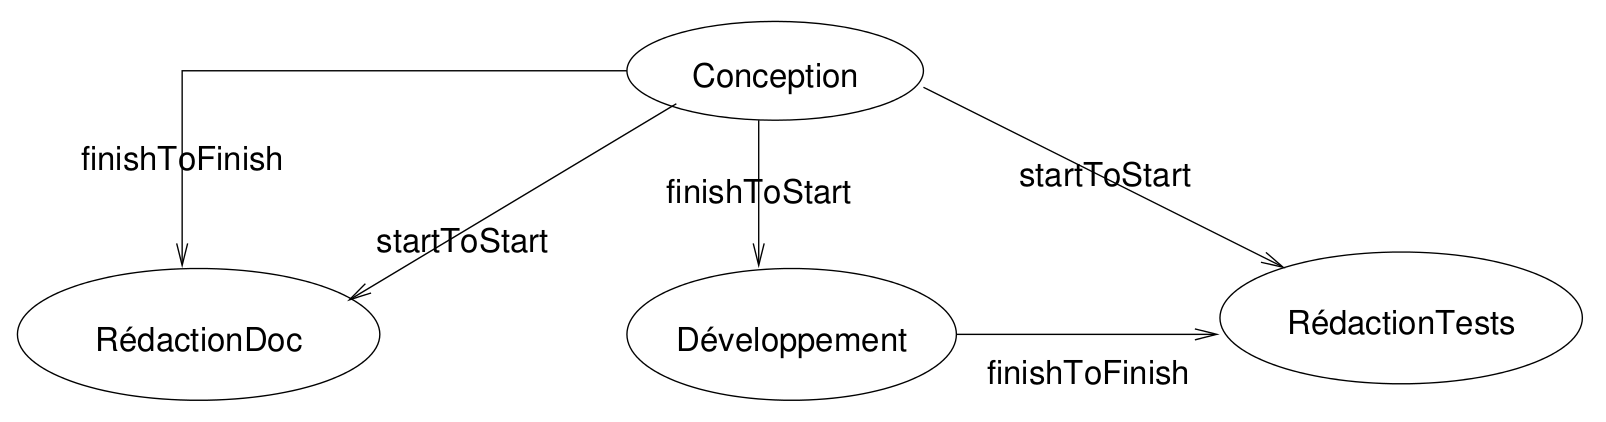
\includegraphics[width = 0.6\textwidth]{../Images/tp2/tp2_2-1.png}}
   \subfloat[Process.xmi]{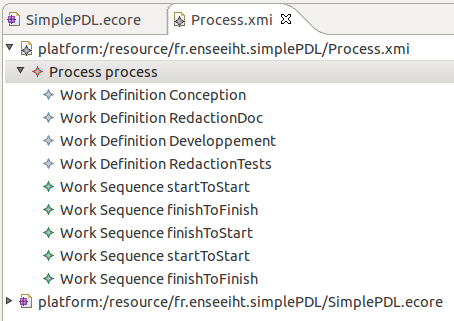
\includegraphics[width = 0.4\textwidth]{../Images/tp2/tp2_2-2.png}}
   \caption{Exemple de modèle de procédé}
   \label{process-1}
\end{figure}

\section{Compléter le métamodèle de SimplePDL}

On propose de compléter un peu le métamodèle de SimplePDL en ajoutant des \textit{ProcessElement} regrougant les \textit{WorkDefinition} et les \textit{WorkSequence} ainsi que d'ajouter la notion de \textit{Guidance} :

\begin{figure}[h]
   \centering
   \subfloat[Ancien modèle]{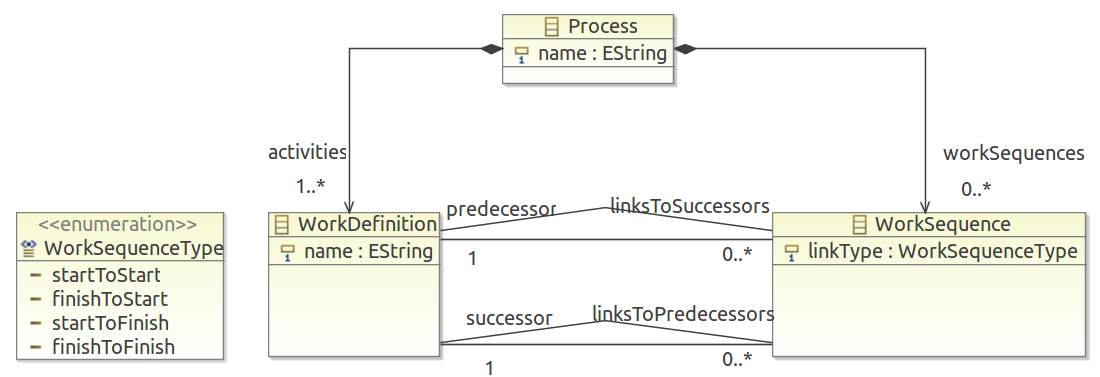
\includegraphics[width = 0.5\textwidth]{../Images/tp2/tp2_1-2.png}}
   \subfloat[Nouveau modèle]{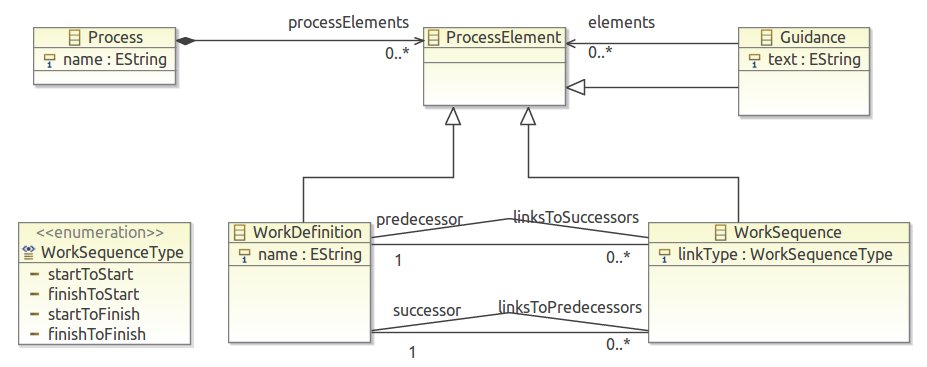
\includegraphics[width = 0.5\textwidth]{../Images/tp2/tp2_3-2.png}}
   \caption{Nouveau métamodèle de SimplePDL}
   \label{pdlv2}
\end{figure}

Le nouveau modèle permet d'ajouter plus de souplesse et de factoriser les propriétés communes aux éléments que l'on pourrait ajouter plus tard. Par contre cette factorisation regroupe l'ensemble des éléments sous le terme générique \textit{processElements} alors qu'on pouvait préciser avant \textit{activities} et \textit{WorkSequences}.

\section{Définir un métamodèle des réseaux de Petri}

On se propose maintenant de définir un métamodèle pour les réseaux de Petri.

\begin{figure}[h]
   \centering
   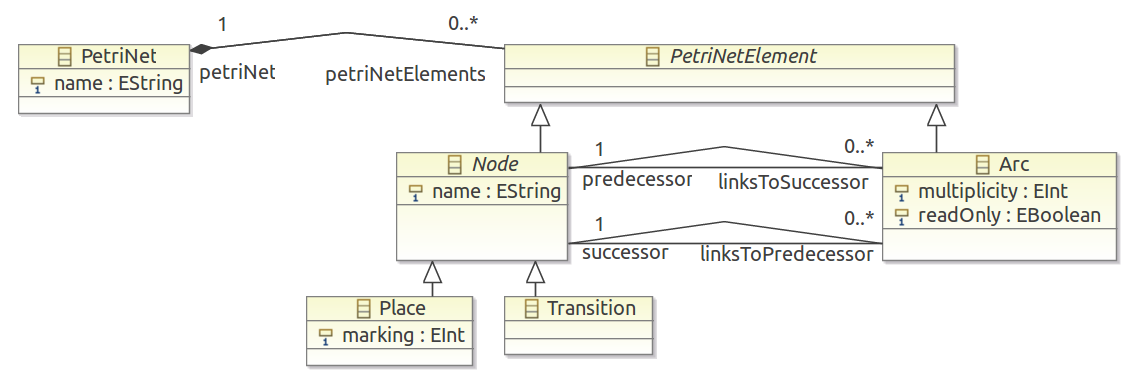
\includegraphics[width = 0.8\textwidth]{../Images/tp2/tp2_4.png}
   \caption{proposition de modèle pour les réseaux de Petri}
   \label{petriModel}
\end{figure}

Ce métamodèle est plus général que celui des réseaux de Petri. Un modèle suivant ce métamodèle peut par exemple avoir un arc reliant 2 places ou 2 transitions ce qui ne devrait pas être possible pour un réseau de Petri. On pourra cependant donner des restrictions et des règles avec le langage OCL pour ne décrire que des réseaux de Petri.
